\documentclass[mathserif,handout]{beamer}

\usepackage{amsmath}
\usepackage{amsfonts}
\usepackage{amssymb}
\newcommand{\ket}[1]{\left| #1\right\rangle}
\newcommand{\bra}[1]{\left\langle #1\right|}
\newcommand{\projector}[1]{\ket{#1}\!\!\bra{#1}}
\newcommand{\braket}[2]{\left \langle #1 \right|\left.\! #2\right\rangle}
\newcommand{\tr}{\mathrm{tr}}
\newcommand{\kpsi}{\ket{\psi}}
\newcommand{\ppsi}{\projector{\psi}}
\newcommand{\bbone}{\ensuremath{\resizebox{5pt}{5.8pt}{1}\hspace{-3.5pt}1}}
\usepackage[all]{xy}

\setbeamercolor{eecks} {bg=Burlywood3, fg=RoyalBlue3}
\newcommand{\defeq}{\overset{\mathrm{def}}{=}}

\author{Alejandro Agust\'{i} Mart\'{i}nez-Soria Gallo}
\title{About the joint measurability of observables}

\begin{document}

\begin{frame}
\maketitle
\end{frame}


\begin{frame}
\tableofcontents


\end{frame}


\begin{frame}
\frametitle{Projector valued measures (PVM)}
\section{Introduction to measures}


\begin{itemize}
\item<1-> Self-adjoint operators as observables:
$$\mathbf{A} \longleftrightarrow \hat{A} = \sum_{i=1}^{n} \alpha_{i}\projector{\alpha_{i}}$$
\item<2-> Probabilities for each state $\kpsi$:
$$\kpsi \longrightarrow p(\alpha_{i}) =  \braket{\alpha_{i}}{\psi}\braket{\psi}{\alpha_{i}} = \tr \left (\projector{\alpha_{i}}\ppsi\right )$$
\item<3-> Together, they provide the conditions:
$$
\hat{A} \longleftrightarrow  \{ \projector{\alpha_{1}} ,\ldots , \projector{\alpha_{n}}  \} 
$$
$$
\projector{\alpha_{i}} \geq 0 
\textcolor{gray}{\Longleftrightarrow \bra{\psi} \projector{\alpha_{i}}\kpsi \geq 0, \forall \kpsi}
$$
$$
\sum_{i}\projector{\alpha_{i}}  = \bbone, \qquad \sum_{i}p(\alpha_{i} ) = 1, \forall \kpsi
$$
\end{itemize}
\end{frame}


\begin{frame}
\frametitle{Positive operator valued measures (POVM)}

\begin{itemize}
\item We need $\{E_{1}, \ldots , E_{n}\}$ such that :
$$
E_{i}\geq 0\qquad\mbox{and}\qquad \sum_{i=1}^{n}E_{i} =\bbone
$$
\item Outcomes optional, $\Omega = \{\omega_{1}, \ldots , \omega_{n}\}$, 
$$
\omega_{i} \overset{\mathsf{E}}{\longmapsto} E_{i}
$$
\item E.g.    
$$
\mathsf{E}(\omega_{i}) = E_{i}, \qquad \mathsf{E}(\omega_{i}, \omega_{j}) = E_{i} + E_{j} , \qquad
\ldots
$$
\item \textcolor{blue}{\bf Origin:} Measuring an observable of a system $S$ on a subsystem $A$ \textcolor{gray}{\it (partial trace, \ldots )}. 
\end{itemize}
\end{frame}







\begin{frame}
\section{Joint measurability of POVM}
\frametitle{Joint measurability of POVM}

\begin{center}
$\{A_{1}, \ldots , A_{n}\}\qquad \{B_{1}, \ldots , B_{m}\}$ 
\end{center}

\begin{itemize}[<+->]
\item Joint POVM
$$
\{ R_{ij} \mid i\in\{1, \ldots , n\}, j \in \{1, \ldots , m\}  \}
$$
\item We get the former POVM's out of $\mathsf{R}$, 
$$
A_{i} = \sum_{j= 1}^{m}R_{ij} \qquad B_{j}  = \sum_{i=1}^{n}R_{ij}
$$
\item In the projective case, $A_{i} = \projector{\alpha_{i}}$, $B_{j} = \projector{\beta_{j}}$. Then $\forall i ,j$
$$
\big [\projector{\alpha_{i}} ,\projector{\beta_{j}}\big ] = 0
 \Rightarrow 
 R_{ij}
 \defeq 
 \overbrace{\projector{\alpha_{i}}}^{A_{i}}
 \underbrace{\projector{\beta_{j}}}_{B_{j}}
 \geq 0
$$ 
\end{itemize}


\end{frame}

%\begin{frame}
%\frametitle{Noise model}
%\framesubtitle{Adding noise to induce joint measurability}
%\end{frame}


\begin{frame}
\section{ Joint measurability of two outcome POVMs}
\frametitle{ Joint measurability of two outcome POVMs }
\framesubtitle{Case for two POVMs}
We have $\{P, \bbone - P\}$ and $\{Q, \bbone - Q\}$ with \emph{outcome spaces} $\{+,-\}$. There exists an $S$ such that 
$$
\begin{matrix}
\bbone - P - Q + S \geq 0 \\
P - S \geq 0 \\
Q -S \geq 0 \\
S\geq 0 
\end{matrix}
\Longleftrightarrow
\begin{matrix}
R_{++}= S \\
R_{-+}= Q - R_{++}\\
R_{+-}= P - R_{++}\\
R_{--} = \bbone - P - Q + R_{++}
\end{matrix}
$$


\end{frame}

\begin{frame}
\frametitle{ Joint measurability of two outcome POVMs }
\framesubtitle{Case for two POVMs: \textcolor{red}{Semi-definite program (SDP)}}
\textit{Remember}: We have $\{P, \bbone - P\}$ and $\{Q, \bbone - Q\}$. 
$$\left .
\begin{matrix}
\inf\tilde \lambda \\
\mbox{\color{red}subjected to }\\
\tilde\lambda\bbone - P - Q + S \geq 0 \\
P - S \geq 0 \\
Q -S \geq 0 \\
S\geq 0 
\end{matrix}
\right \} \rightarrow 
\begin{matrix}
\mbox{\underline{\it \color{blue}Semi-definite program}}\\
\\
 \lambda \leq 1 \Leftrightarrow \mbox{Joint measurability} \\
 \lambda > 1 \Leftrightarrow \neg\mbox{Joint measurability} 
\end{matrix}
$$


\begin{alertblock}{\bf Proposition\footnote{\tiny M. Wolf, D. Perez-Garcia, C. Fern\'{a}ndez . Phys. Rev. Lett., 103:230402, Dec 2009.}}
Let $\lambda $ and $S_{0}$ be the solutions of the SDP above. The parameter $\eta = \max\{0, 1 - \lambda^{-1}\}$ is the least such that the POVMs $(1-\eta) P + \eta E$ and $(1-\eta) Q + \eta E$ are jointly measurable \textcolor{red}{for every} $E$ fulfilling $0\leq E\leq \bbone$. 
\end{alertblock}


\end{frame}


\begin{frame}{Route plan}
How do we correct the mistake and provide for a generalization of the parameter? 
\begin{itemize}
\item Similar but consistent choice of parameters.
\item Developement of geometrical and notational framework to circumvent the difficulties of the generalization (\textit{Graphs}).
\item Mathematically search for viable properties of these geometrical structures (\textit{subgraphs\ldots})
\end{itemize}

\end{frame}


\begin{frame}{Joint measurability graphs}{Joint measurability graph for two POVMs}
\section{Joint measurability graphs}
$$
\xymatrix@ C = 4mm{
\mathbf{0}&&\lambda\bbone\ar[dl]\ar[dr]&\\
\mathbf{1}&P\ar[dr] && Q\ar[dl]\\
\mathbf{2}&&S\ar[d]&\\
&&0&
}\Longleftrightarrow
\xymatrix{
\lambda\bbone - P - Q + S \geq 0 \\
P - S \geq 0,  \quad 
Q -S \geq 0 \\
S\geq 0 
}
  $$

\end{frame}



\begin{frame}{Joint measurability graph for three POVMs}
Let us have $\{P_{i}, \bbone - P_{i}\}$ where $i\in \mathcal{N} = \{1,2,3\}$. 
\begin{figure}[h]
$$
\xymatrix@C=2mm{
\mathbf{0}&&&&S(\emptyset) \ar[dl]\ar[dr]\ar[d]&&&\\
\mathbf{1}&&&S(1)\ar@{-->}[dr]\ar[d]&S(2)\ar[dl]\ar[dr]&S(3)\ar[d]\ar@{-->}[dl]&&\\
\mathbf{2}&&&S(1,2)\ar[dr]&S(1,3)\ar@{-->}[d]&S(2,3)\ar[dl]&&\\
\mathbf{3}&&&&S(1,2,3)\ar[d]&&&\\
&&&&0&&&\\
}
$$
\caption{Joint measurability graph for $n=3$.}
\label{fig:graph_n_3}
\end{figure}


\end{frame}


\begin{frame}{Joint measurability for three POVMs}{Refinement result}
\begin{alertblock}{\color{red} \bf Proposition refined}
$\lambda$ is the least number such that $(1-\eta)P_{i}$ for $i\in\{1, \ldots , n\}$ are jointly measurable. Also if $\lambda \bbone - P_{1}-P_{2}- P_{3}- \ldots \neq 0$ then there exist operators $0\leq E \leq \bbone$ such that $(1-\eta)P_{i} + \eta E$ are jointly measurable, where $\eta = \max\{0, 1-\lambda^{-1}\}$. 
\end{alertblock}
$$
\resizebox{.45\textwidth}{!}{\xymatrix@C=2mm{
&&&\lambda \bbone\ar[dl]\ar[dr]\ar[d]&&&\\
&&P_{1}\ar@{-->}[dr]\ar[d]&P_{2}\ar[dl]\ar[dr]&P_{3}\ar[d]\ar@{-->}[dl]&&\\
&&S(1,2)\ar[dr]&S(1,3)\ar@{-->}[d]&S(2,3)\ar[dl]&&\\
&&&S(1,2,3)\ar[d]&&&\\
&&&0&&&\\
}
}
\xymatrix@R=1mm{
\mbox{We can make $\lambda$ in the proposition }\\
\mbox{independent on the choice of $P_{i}$, by } \\
\mbox{taking the maximum over all }\\
\mbox{combinations of POVM elements.}
}
$$

\end{frame}

\begin{frame}{Joint measurability for three POVMs}{Subgraphs}
$$\xymatrix@C=2mm{
&&&\textcolor{red}{\lambda_{2} }\bbone\ar@[red][dl]\ar@[gray][dr]\ar@[red][d]&&&\\
&&P_{1}\ar@[gray][dr]\ar@[red][d]&P_{2}\ar@[red][dl]\ar@[gray][dr]&P_{3}\ar@[gray][d]\ar@[gray][dl]&&\\
&&S(1,2)\ar@{-->}@[red]@/^-1pc/[ddr]\ar@[gray][dr]&S(1,3)\ar@[gray][d]&S(2,3)\ar@[gray][dl]&&\\
&&&S(1,2,3)\ar@[gray][d]&&&\\
&&&0&&&\\
}
$$
\end{frame}



\begin{frame}{Joint measurability for three POVMs}{Parameter tree}

$$\xymatrix@C=2mm{
&&\lambda \bbone\ar[dl]\ar[dr]\ar[d]&&&\\
1\ar@{}[d]|{\color{red}\vee /}&P_{1}\ar@{-->}[dr]\ar[d]&P_{2}\ar[dl]\ar[dr]&P_{3}\ar[d]\ar@{-->}[dl]&&\\
\textcolor{blue}{\eta_{2}}\ar@{}[d]|{\color{red}\vee /}&S(1,2)\ar[dr]&S(1,3)\ar@{-->}[d]&S(2,3)\ar[dl]&&\\
\textcolor{blue}{\eta_{3}}\ar@{}[d]|{\color{red}\vee /}&&S(1,2,3)\ar[d]&&&\\
0&&0&&&\\
}$$


\end{frame}


\begin{frame}

\begin{center}
\bf 
Thank you very much 
\begin{center}
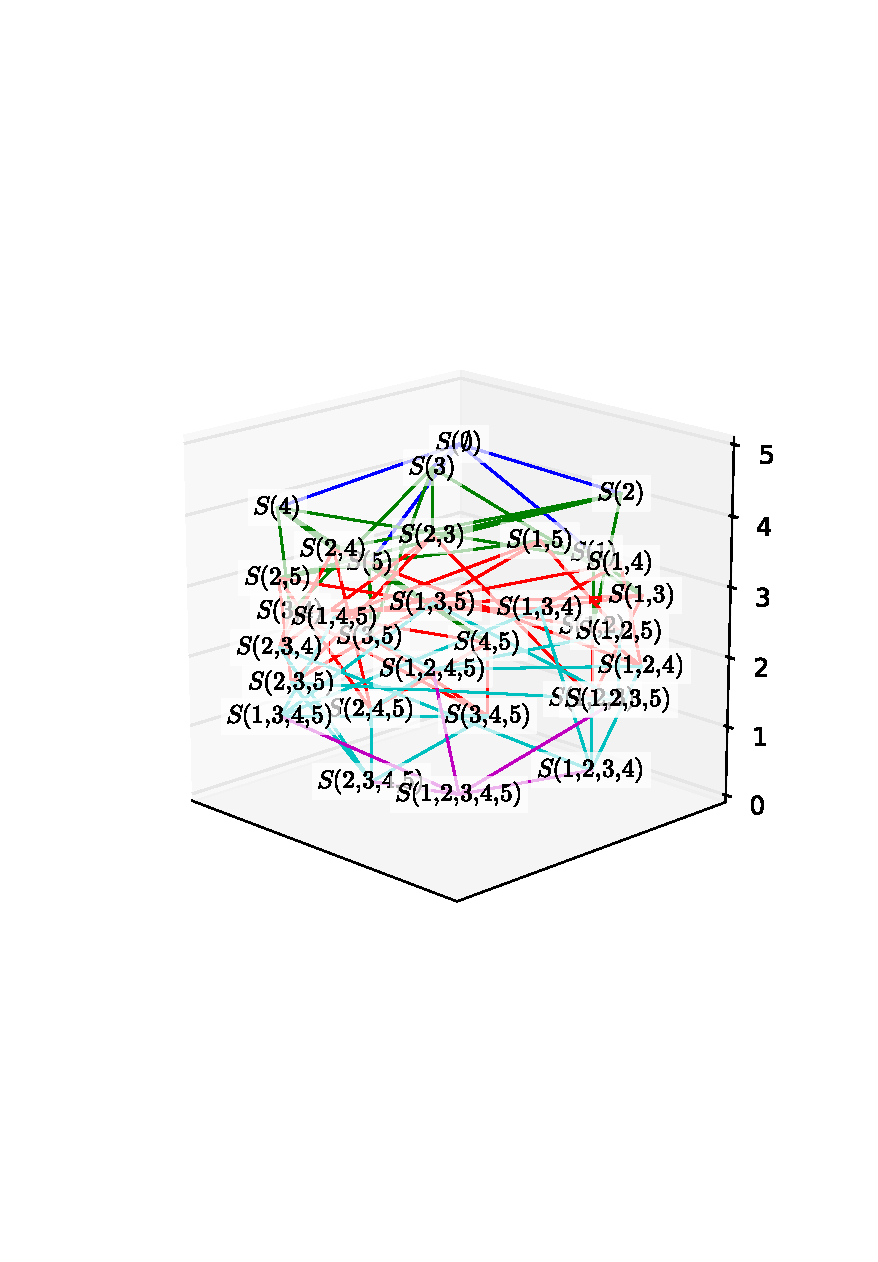
\includegraphics[scale=.6]{images/6.pdf}
\end{center}
for your attention! 
\end{center}
\end{frame}


\end{document}